\chapter{PyBEL}
\label{ch:pybel}

\section{Survey of Current Technologies}

While there exist several software packages for \ac{BioPAX} and \ac{SBML}, the ecosystem of open-source software for \ac{BEL} is much more limited.

\subsection{OpenBEL Framework}

With its publication of the \ac{BEL} v1.0 specification as an open standard, the OpenBEL Consortium released the OpenBEL Framework \cite{openbelframework} ; a Java framework for parsing BEL v1.0 documents and its companion Cytoscape plugin \cite{openbelframeworkcytoscapeplugins} for network visualizations.

\subsection{bel.rb}
Ongoing development slowed \cite{openbelframeworkgraphs} as the focus of OpenBEL development shifted towards \verb|bel.rb| \cite{belrb}; a Ruby tool for parsing and transforming BEL v1.0 Script to \ac{RDF}. Additionally, there is only limited community support through GitHub and the proposed channel on Gitter.

Neither of the previously mentioned softwares provide explicitly documented support for this revision; and the aging codebase of the OpenBEL Framework and the generally low usage of Ruby in the bioinformatics community provide little incentive for updates. 

\section{Motivation}

There is an unmet need for publicly available, easily installable, stable, facile software that parses modern BEL and provides programmatic access to a data container that enables the resulting network to be extended, queried, manipulated, analyzed, and visualized. Furthermore, a converter between common data formats is needed to enable re-usability and interoperability between general and BEL-specific software for network analysis and visualization. This chapter presents PyBEL, a Python language software package designed to fulfill each of these needs.

\section{Software Architecture}

Development of the PyBEL software package adheres to a component-based software architecture. The schematic view in Figure 5 illustrates how data flows between components. components interact to build an integrated environment for working with networks encoded in BEL Script. 

\begin{figure}
\captionsetup{format=plain}
\makebox[\textwidth]{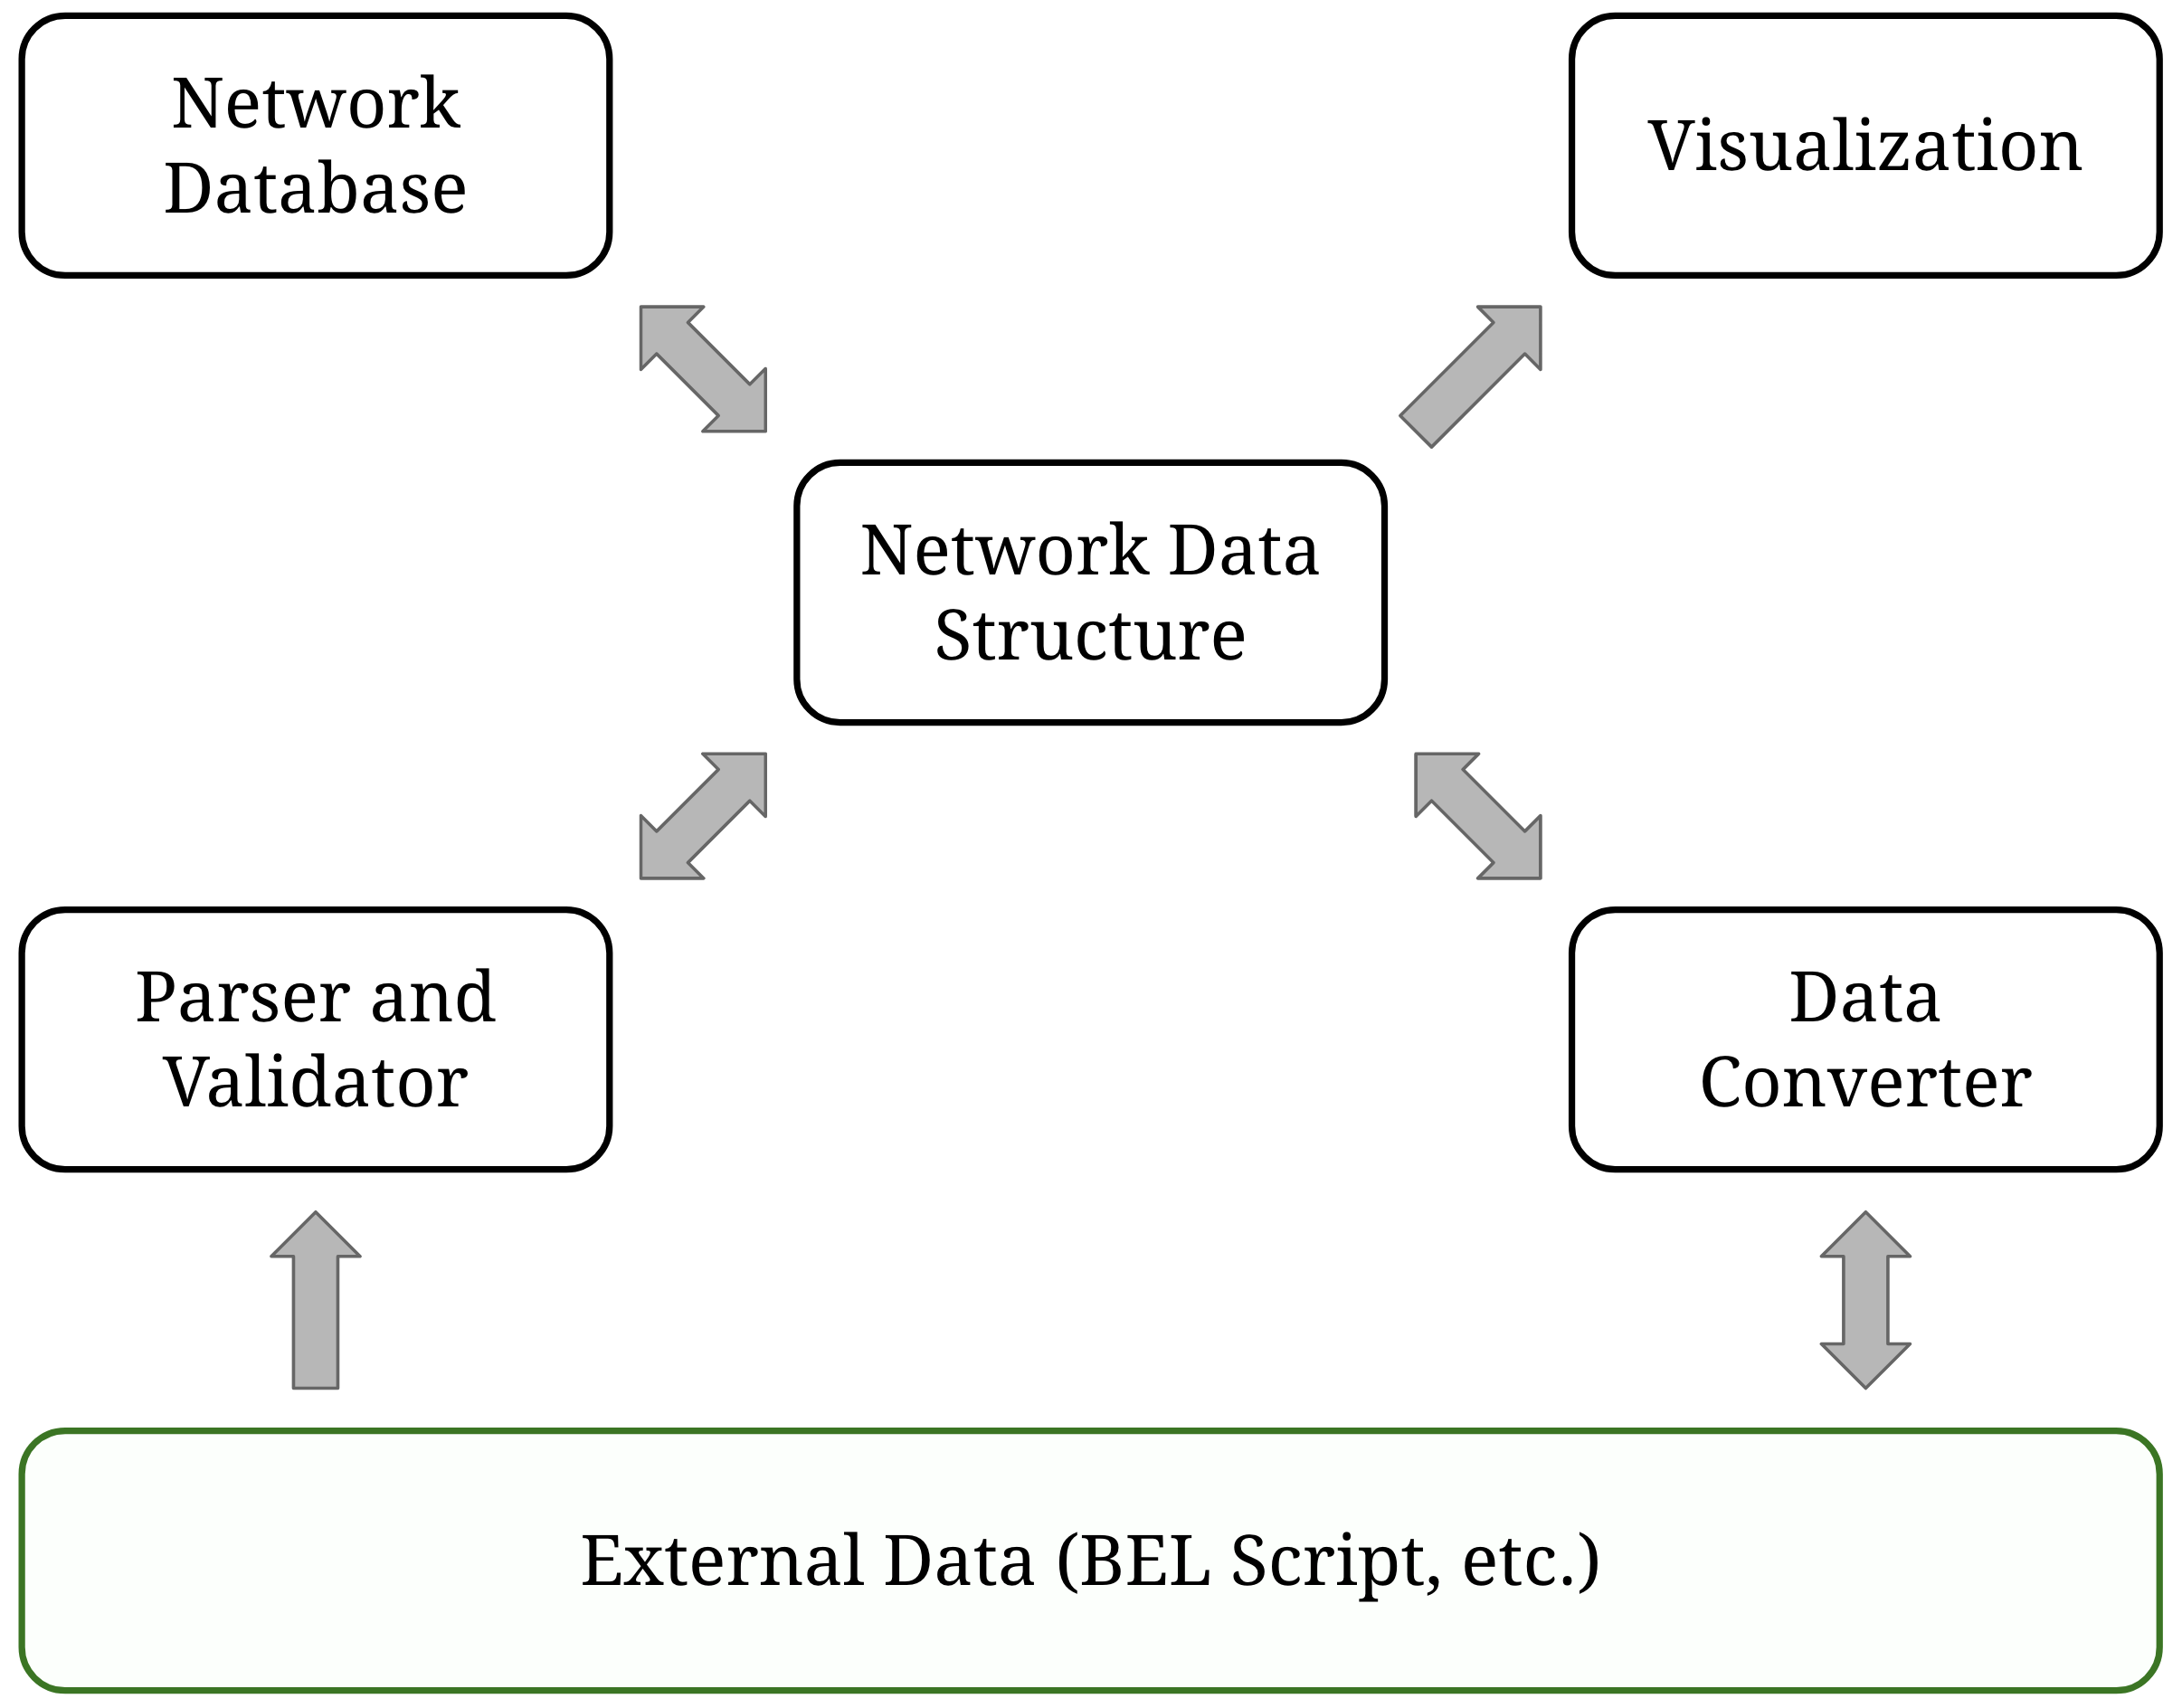
\includegraphics[width=120mm]{images/pybel_components.png}}
\caption[The PyBEL Software Architecture]{The PyBEL software package consists of five main parts: (1) the data container, (2) the parser and validator, (3) the network database, (4) the data converter, and (5) visualization. Arrows represent the direction of the flow of data between components. Together, these components provide a framework for developing tools for exploration and analytics.}
\label{Fig:pybel_components}
\end{figure}

\subsection{Network Data Container}
While a graph refers to an abstraction for a set of objects (i.e. nodes) and their relations (i.e. edges), its instantiation in a real-world application is often called a network. PyBEL implements a directed multigraph (i.e. a graph whose edges have directionality and any given pair of nodes may have multiple edges) that maps the biological entities and concepts in the subjects and objects of \ac{BEL} relations to nodes in a network and their relations, with corresponding metadata, to edges. It extends the MultiDiGraph class from NetworkX, a Python package for manipulation of networks \cite{Hagberg2008}, to enable users direct access to their suite of network algorithms and provide additional tools to develop them into biologically meaningful analyses. While no-SQL database systems like Neo4J \cite{neo4j} are also able to store and make increasingly complicated queries over networks, they inherently lack the extensibility of data structures native to programming languages like Python that can be extended and directly manipulated.

Additional information can be annotated on each of the node, edge, and graph levels. This can allow of the integration of tabular information (i.e. differential gene expression on nodes or $IC_{50}$ values for edges representing inhibition experiments of chemicals on enzymes). Network-level annotations allows for storage of all relevant provenance information related to curation and namespace definitions in order to enable semantic data integration with other network and tabular data sources. 

\subsection{Parsing and Validation}

The parser combines components for performing tokenization, lexical analysis, parsing, and validation on each of the three sections of BEL Script. Each was implemented using the internal domain-specific language provided by the PyParsing \cite{pyparsing} Python package because of its exceptional speed, ease of writing compared to regular expressions, and ability to register callbacks for different language features. One callback annotates the entries in the document metadata section to a network instance while another downloads and stores the resources referenced in the definitions section. The relations section has two main callbacks; one to maintain a list of current annotations from SET statements and another to parse BEL relations (Figure 4C-D) and populate a network instance with the corresponding nodes, edges, and their metadata from the current internal state.  

While relations' syntax is implicitly validated by the implementation of BEL in PyParsing, the semantics of their subjects' and objects' identifiers are validated with the references stored earlier. Finally, feedback is provided to users with thorough error analyses to support thoughtful re-curation, which could lead to more robust knowledge assemblies and enable more reproducible science.

\subsection{Network and Edge Store}

PyBEL uses a relational database to cache external namespaces and pre-parsed networks to improve the speed of validation and access to data. While relational databases are not generally appropriate for applying network algorithms, they do provide indexing functionality that enables complicated queries and filters over the nodes, edges, and metadata of increasingly large collections of networks. For example, this could enable the identification of intersections and potential cross-talk in different disease-specific networks. SQLAlchemy \cite{sqlalchemy}, a popular object-relational mapper, was used to maintain the database schema, transport the results of queries to PyBEL, and enable integration of external relational databases. Additionally, SQLAlchemy supports both fully-featured relational database management systems as well as SQLite \cite{sqlite} for a zero-configuration option. 

\subsection{Data Converter}

Lossless conversion protocols were implemented for common file formats including Node-Link \ac{JSON}, \ac{JGIF}, CX, and Python Pickle as well as for multiple common database formats including \ac{SQL}, Neo4J, and the \ac{NDEx} (Table 1). Additional lossy exporters were provided to \ac{CSV}, \ac{SIF}, Excel, \ac{XGMML}, and \ac{GSEA} and \ac{GRP} to facilitate usage in other programs (Table 2). Notably, implementing a RDF converter was deferred until improvements are made to the existing BEL to RDF mapping and its documentation \cite{openbelrdf}.

\begin{table}
\centering
\caption[PyBEL Interconversion Formats]{Multiple lossless converters are provided to common file formats and databases. Full descriptions of the programmatic API can be found at http://pybel.readthedocs.io/en/latest/io.html}
\label{tab:conversion}
\def\arraystretch{1.5}
\begin{tabular}{p{2cm} p{12cm}}
Format & Usage \\
\hline
BEL Script & Output to BEL scripts results in upgrade of statements from BEL v1.0 and a standardized formatting. \\
Binary & Using Python’s pickle module, pre-parsed BEL Script can be stored as binary data for fast loading, storage in databases, and transfer via network protocols. \\
Node-Link & Node-Link \cite{nodelink} is the standard \ac{JSON} format for many web-based network visualization tools, including D3.js \cite{d3js}. Output is facilitated by standard code provided by NetworkX. \\
JGIF & \ac{JGIF} \cite{jsongraphformat} is defined by a schema that is nearly a proper subset of the Node Link format. Conversion with this format provides compatibility with other software and repositories, such as the Causal Biological Network Database \cite{Talikka2015}. \\
CX & CX \cite{cxmodel} is an aspect-oriented network interchange format encoded in JSON with a format inspired by the JSON-LD \cite{jsonld} encoding of RDF. It is primarily used by the \ac{NDEx} and more recent versions of Cytoscape. \\
NDEx & PyBEL contains wraps the \ac{NDEx} Python client \cite{ndexpython} for seamless upload/download to the \ac{NDEx} in the CX format. \\
SQL & SQLAlchemy is used to make abstract queries over the nodes and edges of a collection of networks. \\
Neo4J & Neo4J  is a graph database that enables complex graph queries with the Cypher querying language.
\end{tabular}
\end{table}

\begin{table}
\centering
\caption[PyBEL Export Formats]{Exporters to lossy and irretrievable formats are provided to promote usability in other programs.}
\label{tab:lossy_exporters}
\def\arraystretch{1.5}
\begin{tabular}{p{2cm} p{12cm}}
Format              & Usage \\
\hline
CSV, SIF, and Excel & \ac{CSV}, \ac{SIF}, and Excel all consist of an edge list with interaction types that are suited for viewing in Excel or Cytoscape.                                                                                              \\
XGMML               & \ac{XGMML} \cite{xgmml} supersedes \ac{GML} by adding support for both node and edge annotations. Its name derives from its encoding in \ac{XML}. It can be directly imported to Cytoscape for viewing. \\
HTML                & Interactive visualizations can be produced using JSON export and D3.js. They can be embedded directly in Jupyter Notebook.                                                                                                                                                  \\
GSEA                & This export option outputs a list of genes in the \ac{GRP} format for use with the Broad Institute’s \ac{GSEA} platform \cite{Subramanian2005}.
\end{tabular}
\end{table}


\subsection{Visualization}

Networks can be exported to \ac{CSV}, \ac{SIF}, \ac{XGMML}, or CX for visualization in Cytoscape \cite{Franz2015} or uploaded to \ac{NDEx} \cite{Pratt2015} to take advantage of its viewer and simple query interface. Alternatively, PyBEL provides an interactive network explorer and visualizer that is tailored to \ac{BEL} networks (appropriate node coloring, metadata pop-ups, etc.) that can be directly embedded as \ac{HTML} in email, Jupyter Notebook \cite{Kluyver2016}, or a web application. For example, it has already been used to produce visualizations in the NeuroMMSig web server \cite{Domingo-Fernandez2017}. Figures 6-8 present the Alzheimer’s Disease Knowledge Assembly Wnt Signaling Subgraph from \ac{NeuroMMSig} in three different visualizations.

\begin{figure}
\captionsetup{format=plain}
\makebox[\textwidth]{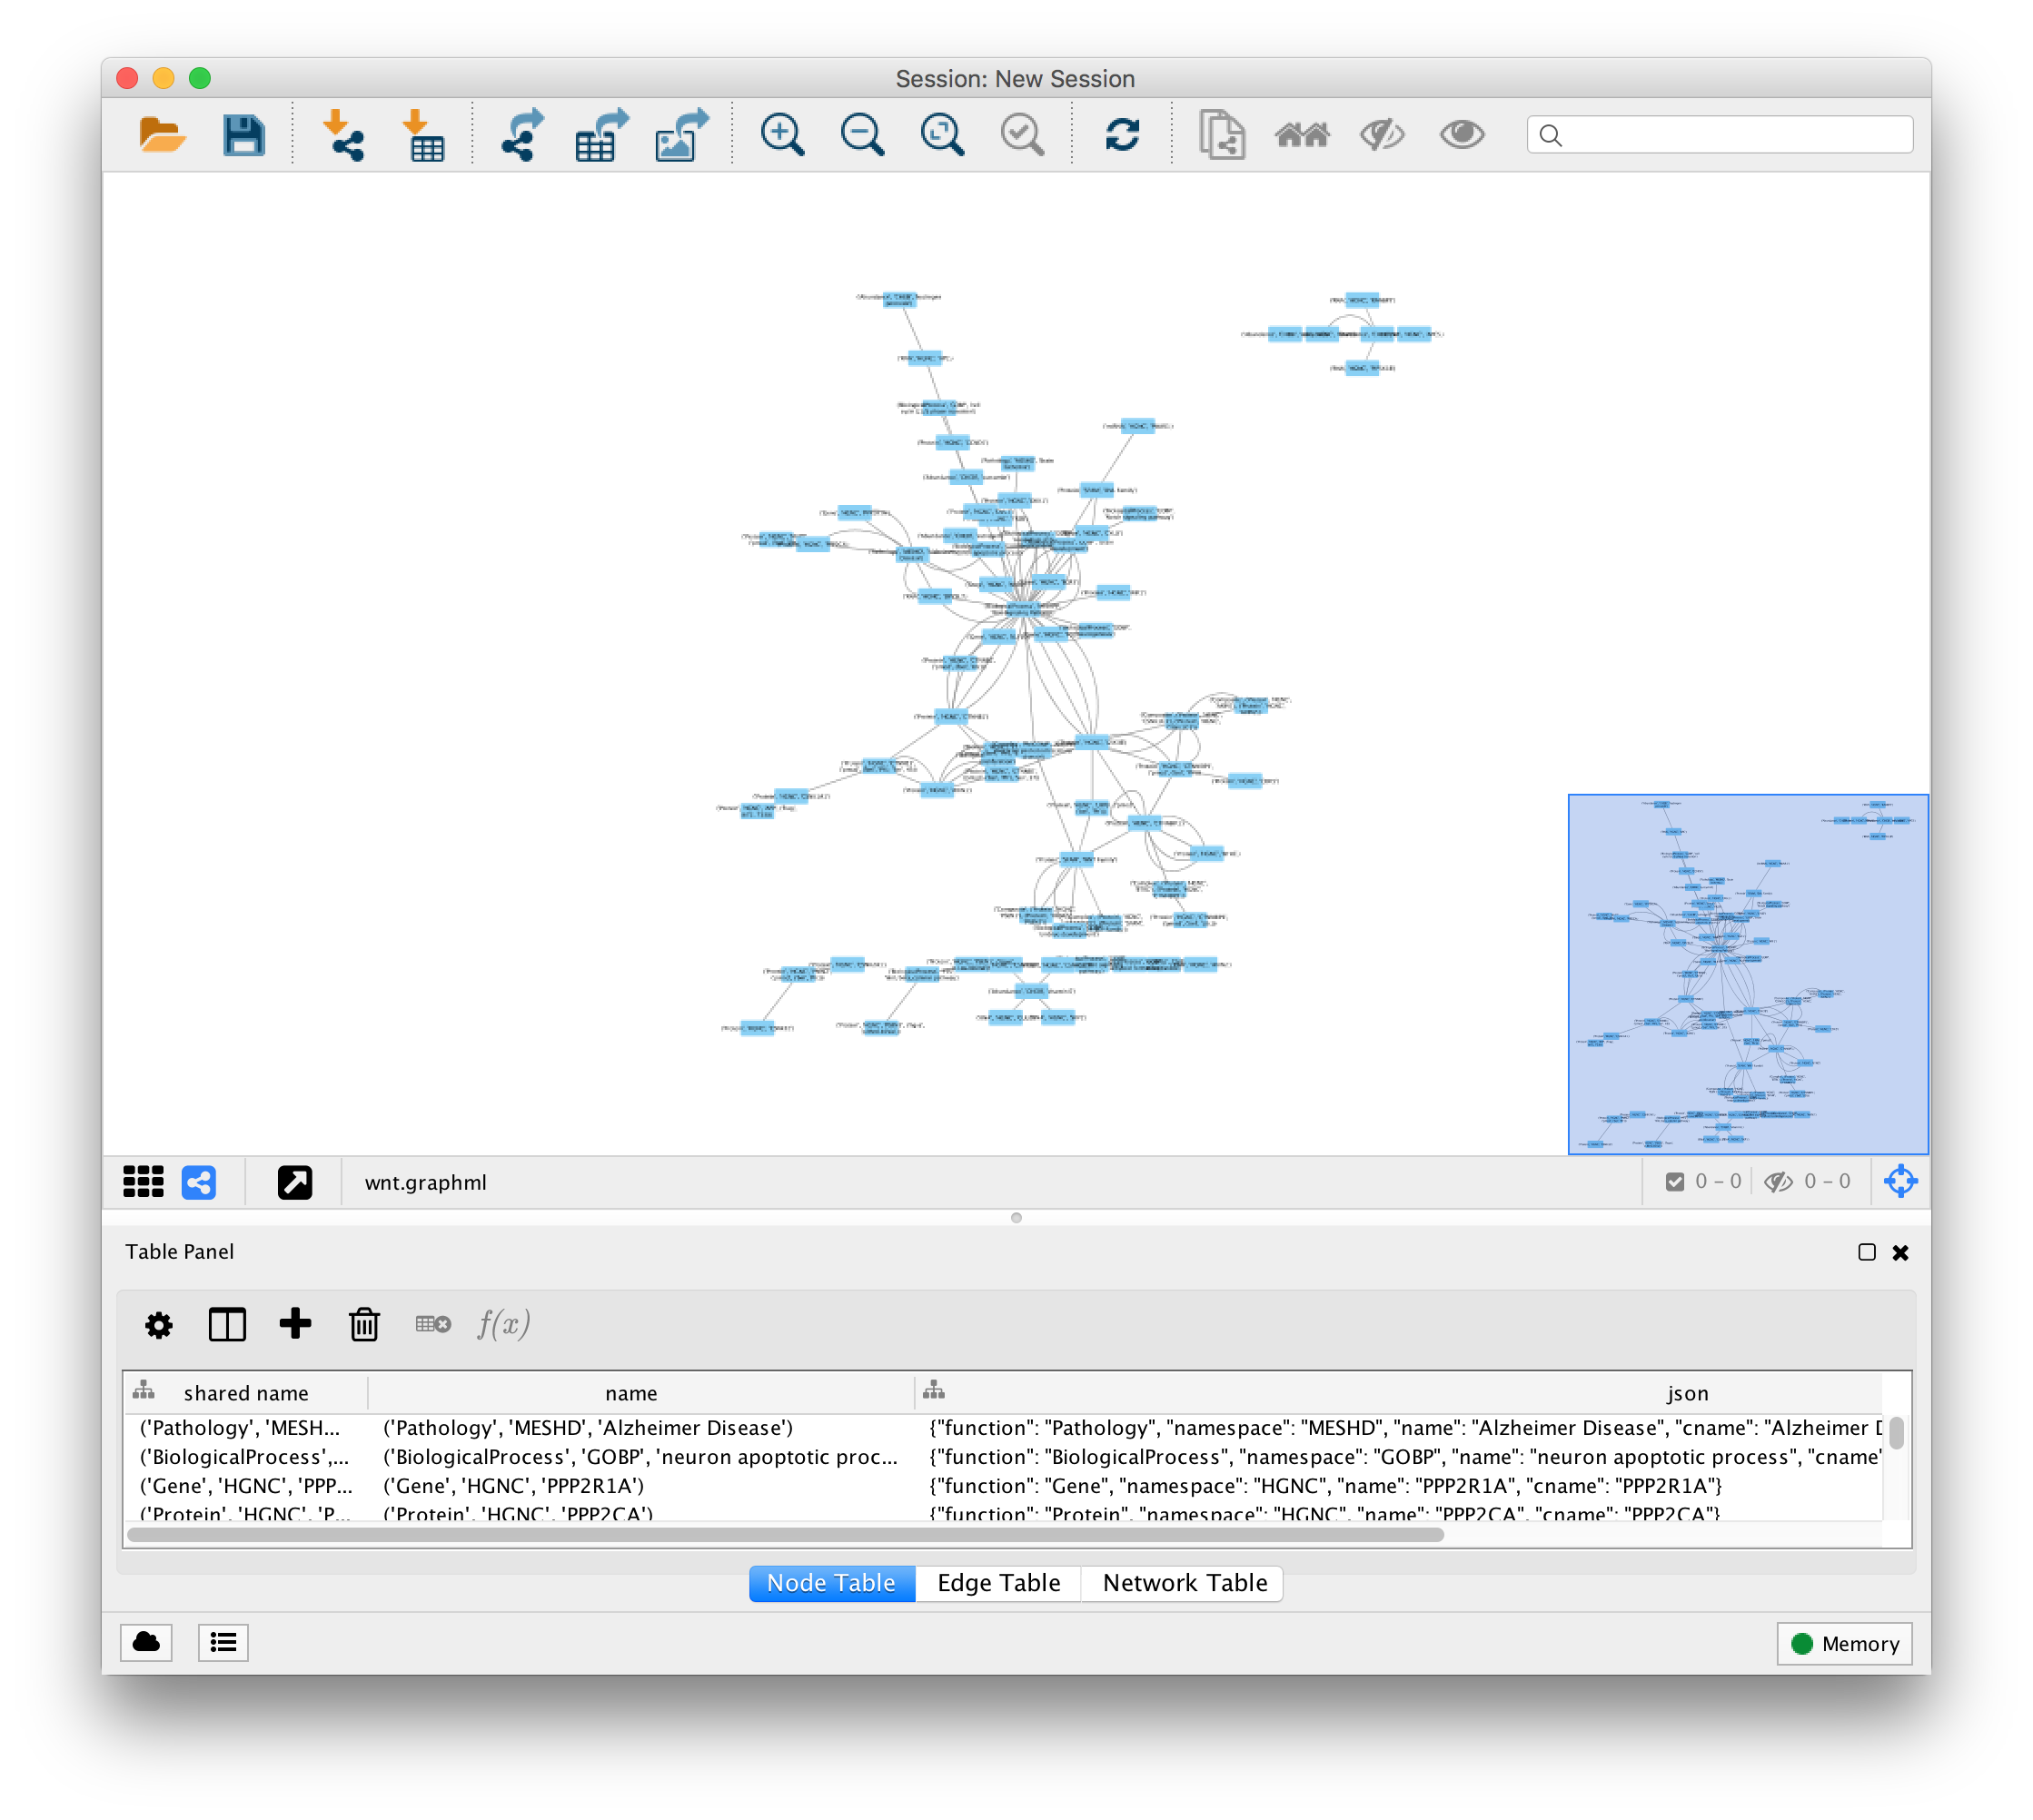
\includegraphics[width=160mm]{images/wnt_cytoscape.png}}
\caption[PyBEL Visualization of Wnt Signaling in Cytoscape]{Visualization of the Wnt Signaling Subgraph from the \ac{NeuroMMSig} Alzheimer’s Disease Knowledge Assembly with Cytoscape provides extensive styling and rudimentary access to the node and edge properties stored in PyBEL. Cytoscape also provides some network analytics functions.}
\label{Fig:wnt_cytoscape}
\end{figure}

\begin{figure}
\captionsetup{format=plain}
\makebox[\textwidth]{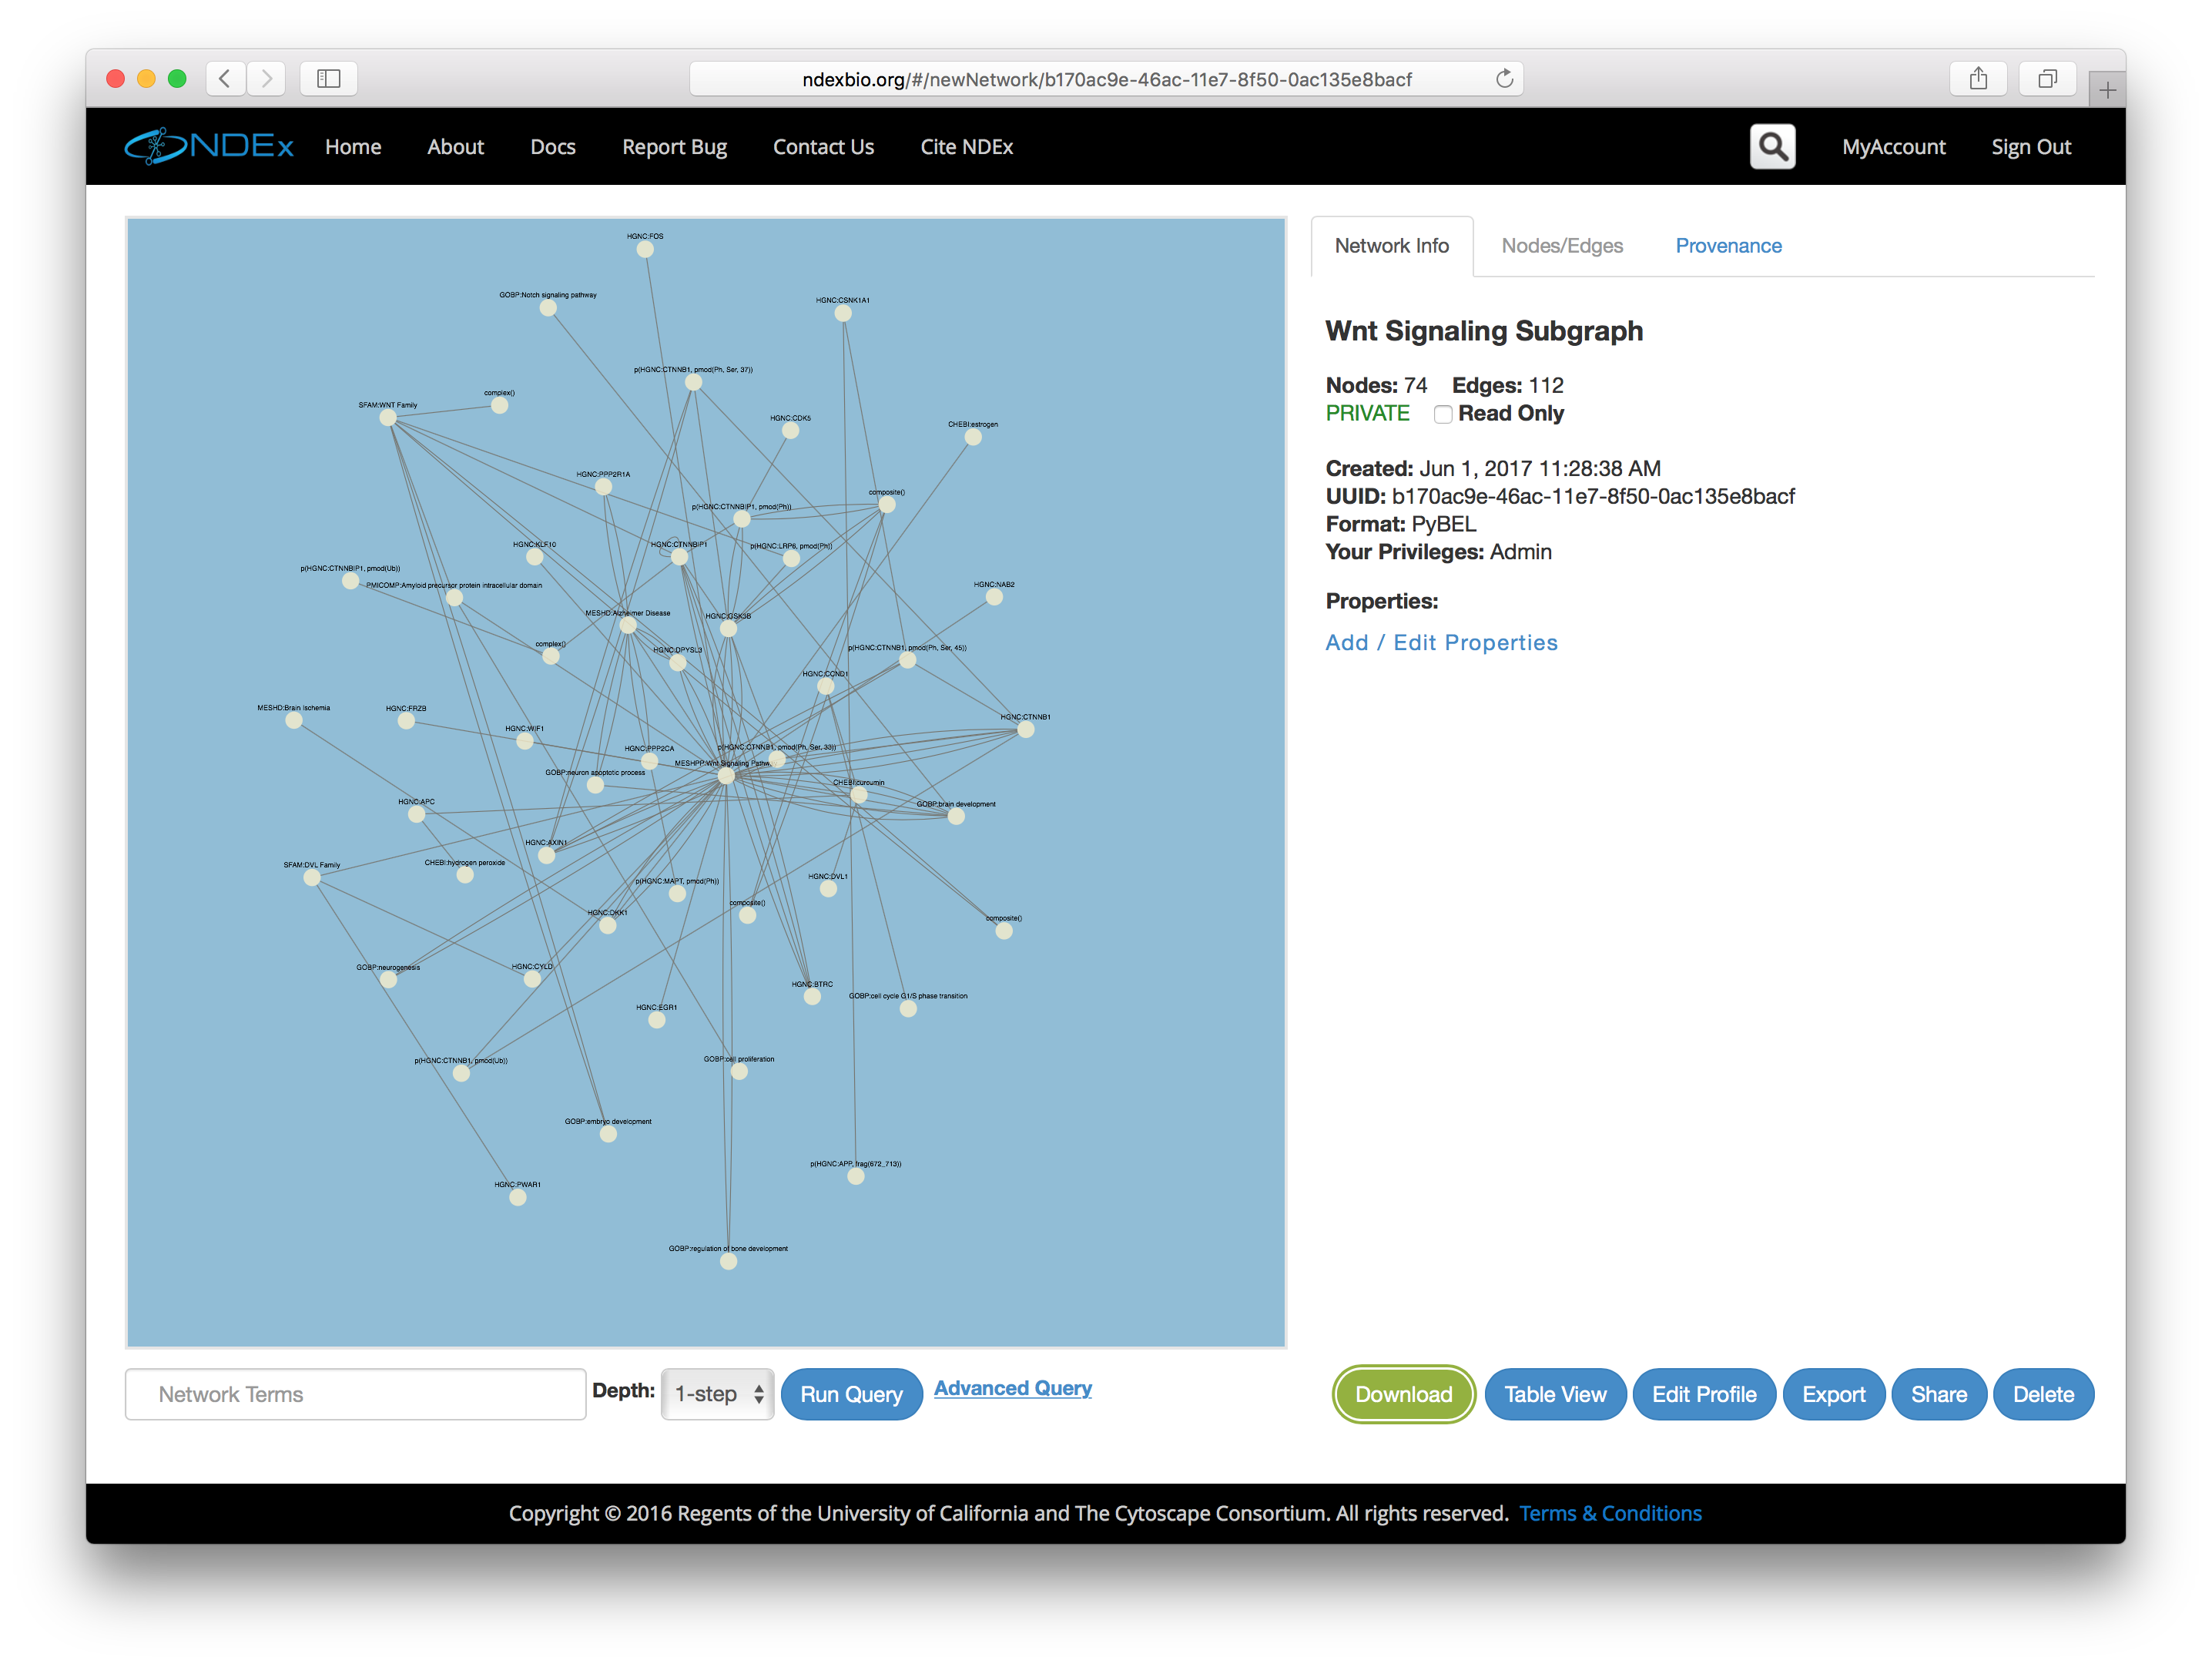
\includegraphics[width=160mm]{images/wnt_ndex.png}}
\caption[PyBEL Visualization of Wnt Signaling in NDEx]{Visualization of the Wnt Signaling Subgraph from the \ac{NeuroMMSig} Alzheimer’s Disease Knowledge Assembly with \ac{NDEx} allows users to easily share their networks.}
\label{Fig:wnt_ndex}
\end{figure}

\begin{figure}
\captionsetup{format=plain}
\makebox[\textwidth]{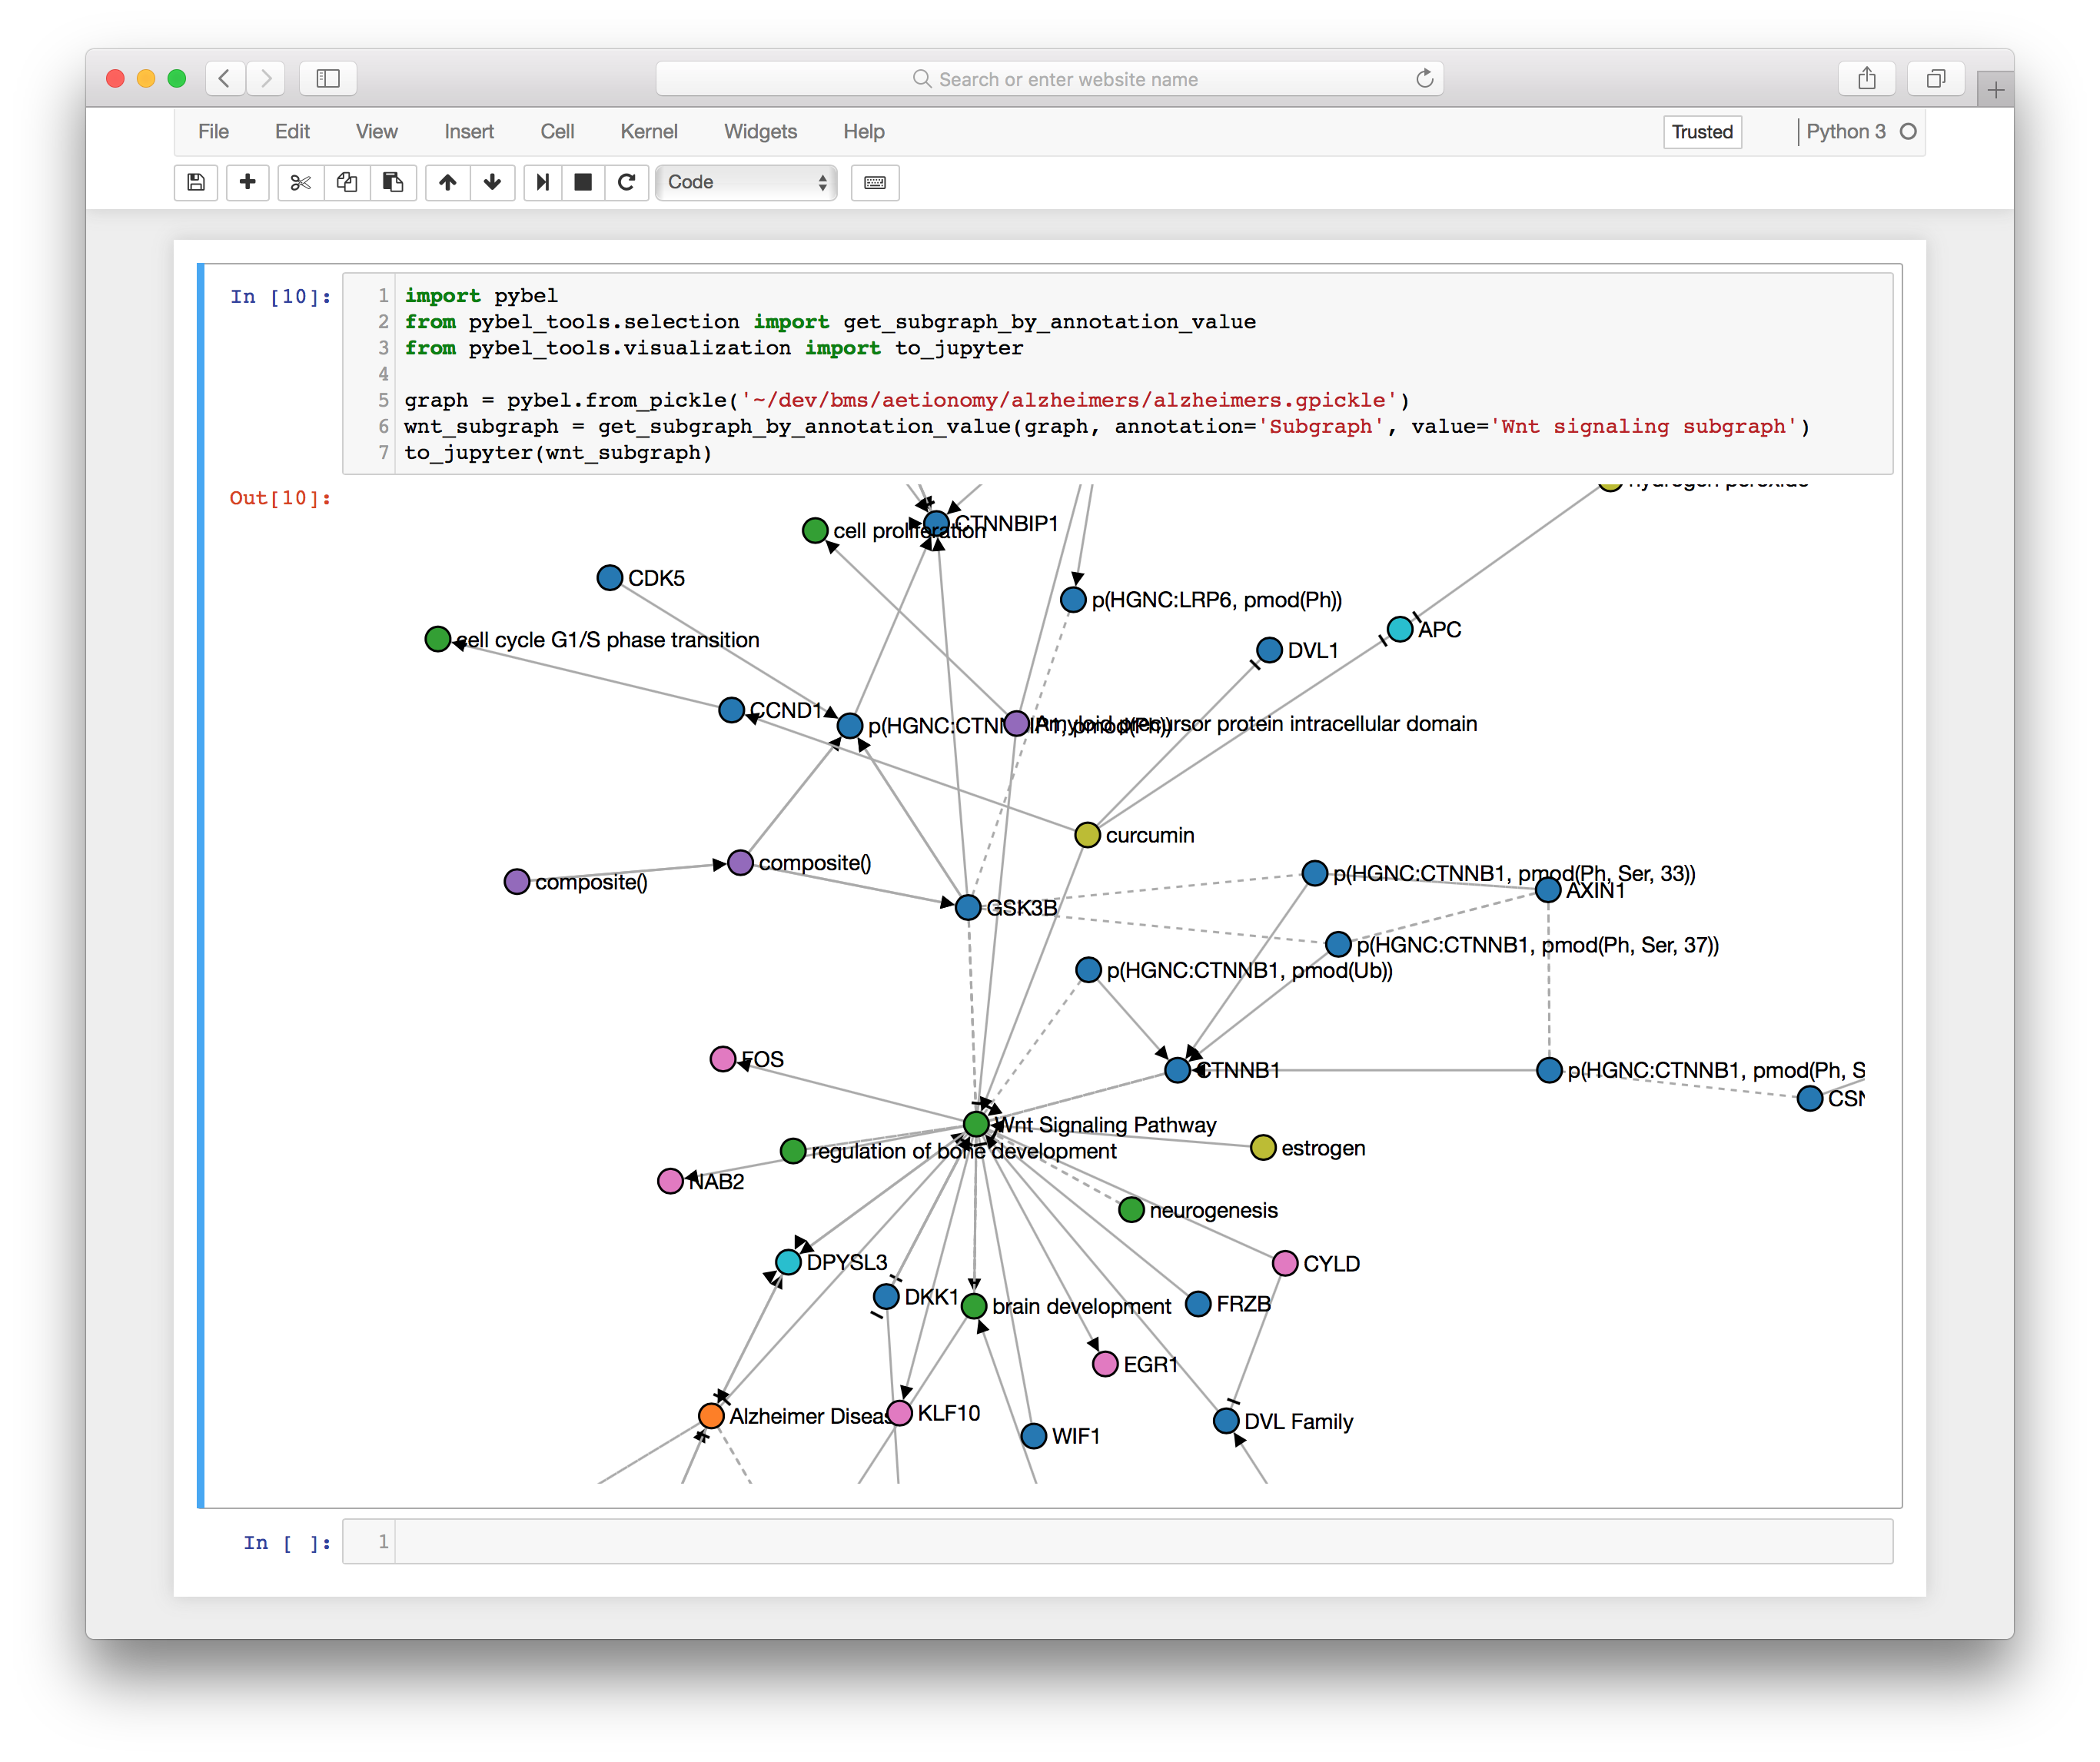
\includegraphics[width=160mm]{images/wnt_jupyter.png}}
\caption[PyBEL Visualization of Wnt Signaling in Jupyter Notebook]{Visualization of the Wnt Signaling Subgraph from the NeuroMMSig Alzheimer’s Disease Knowledge Assembly with Jupyter Notebook allows for embedding within scientific workflows.}
\label{Fig:wnt_jupyter}
\end{figure}

The visualization system from PyBEL has been built in a modular way so it can be integrated in other applications. The underlying Javascript and \ac{HTML} are written with the Jinja templating language \cite{jinja} and exposed via Python functions that can be integrated in Python code or exposed through a RESTful \ac{API}. There is ongoing work to enable users to easily visually explore the results of the \ac{BELIEF} \cite{Madan2016} and \ac{INDRA} \cite{indra} text mining pipelines. Other projects, such as the development of a web service to display and explore a knowledge base assembled for an ongoing project related to \ac{PTSD} are also currently using the PyBEL visualization to embed specific knowledge assemblies with other clinical and molecular data. Figures 9-11 present the PyBEL visualization embedded in other applications that are already in the prototype or release stage of development.

\begin{figure}
\captionsetup{format=plain}
\makebox[\textwidth]{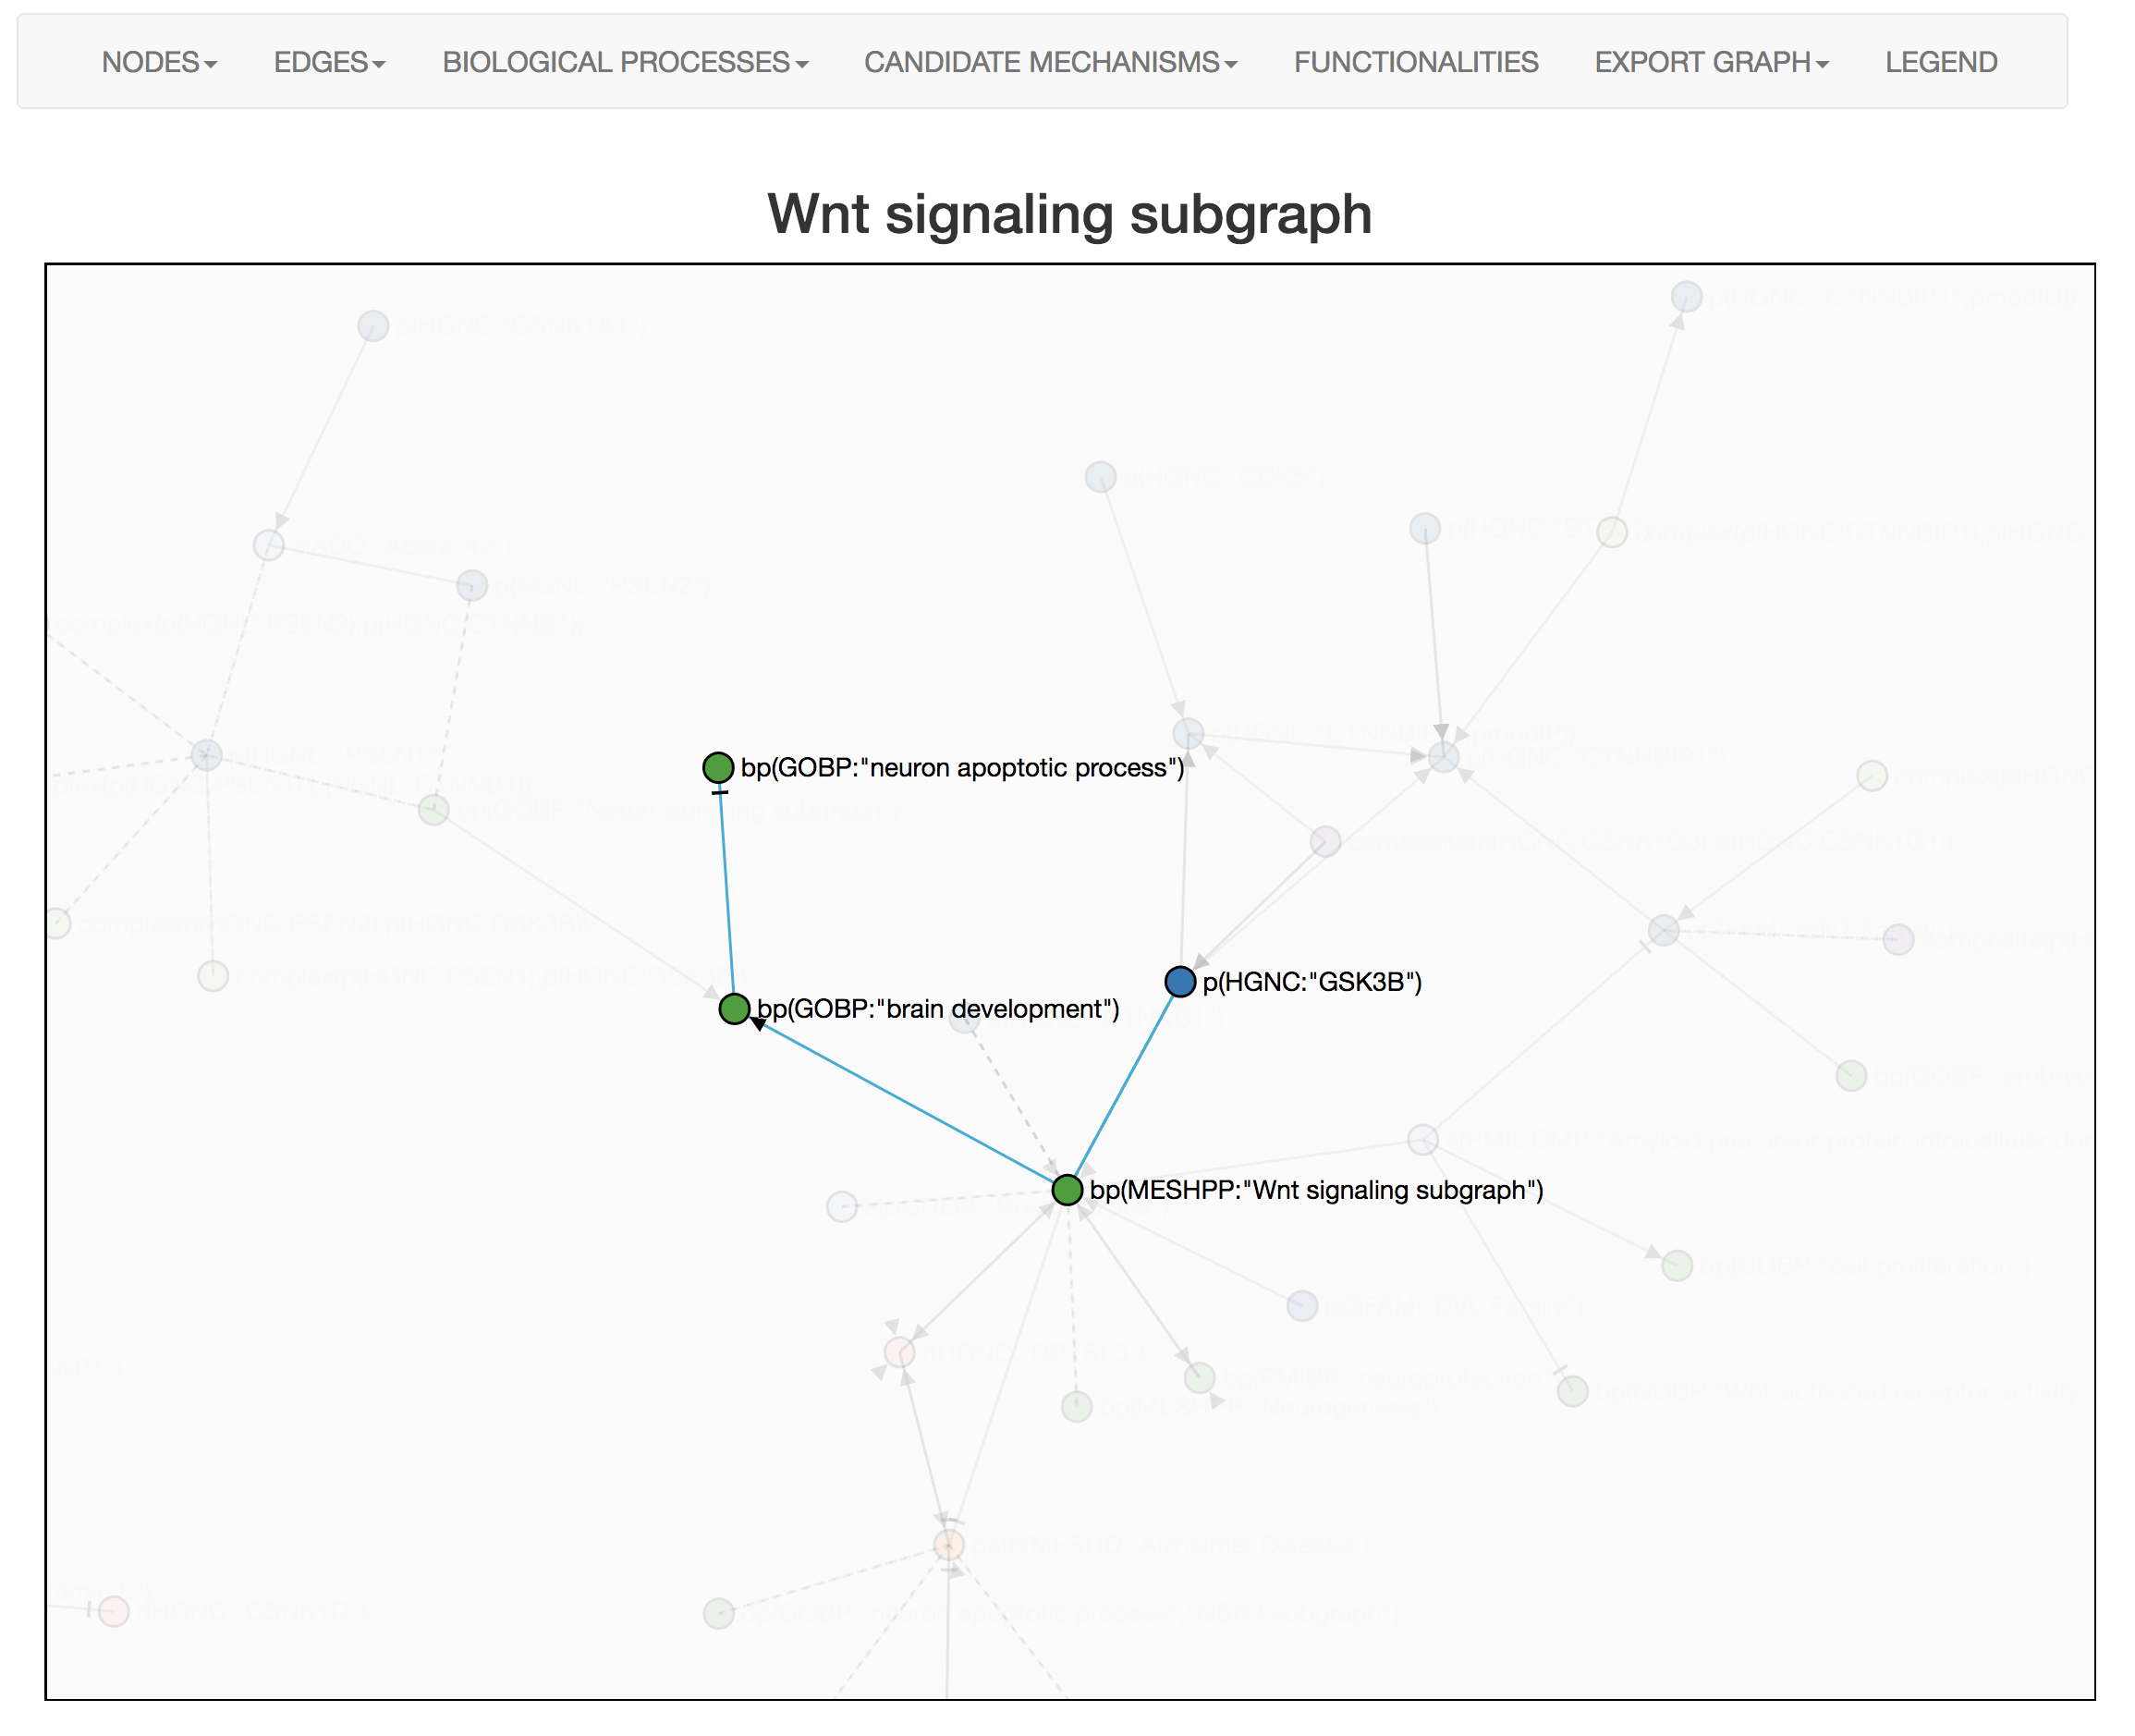
\includegraphics[width=160mm]{images/wnt_neurommsig.png}}
\caption[PyBEL Integration with the NeuroMMSig Mechanism Enrichment Server]{The NeuroMMSig Mechanism Enrichment server uses PyBEL visualization to present a downstream mechanism to the user following multi-modal mechanism enrichment.}
\label{Fig:wnt_neurommsig}
\end{figure}

\begin{figure}
\captionsetup{format=plain}
\makebox[\textwidth]{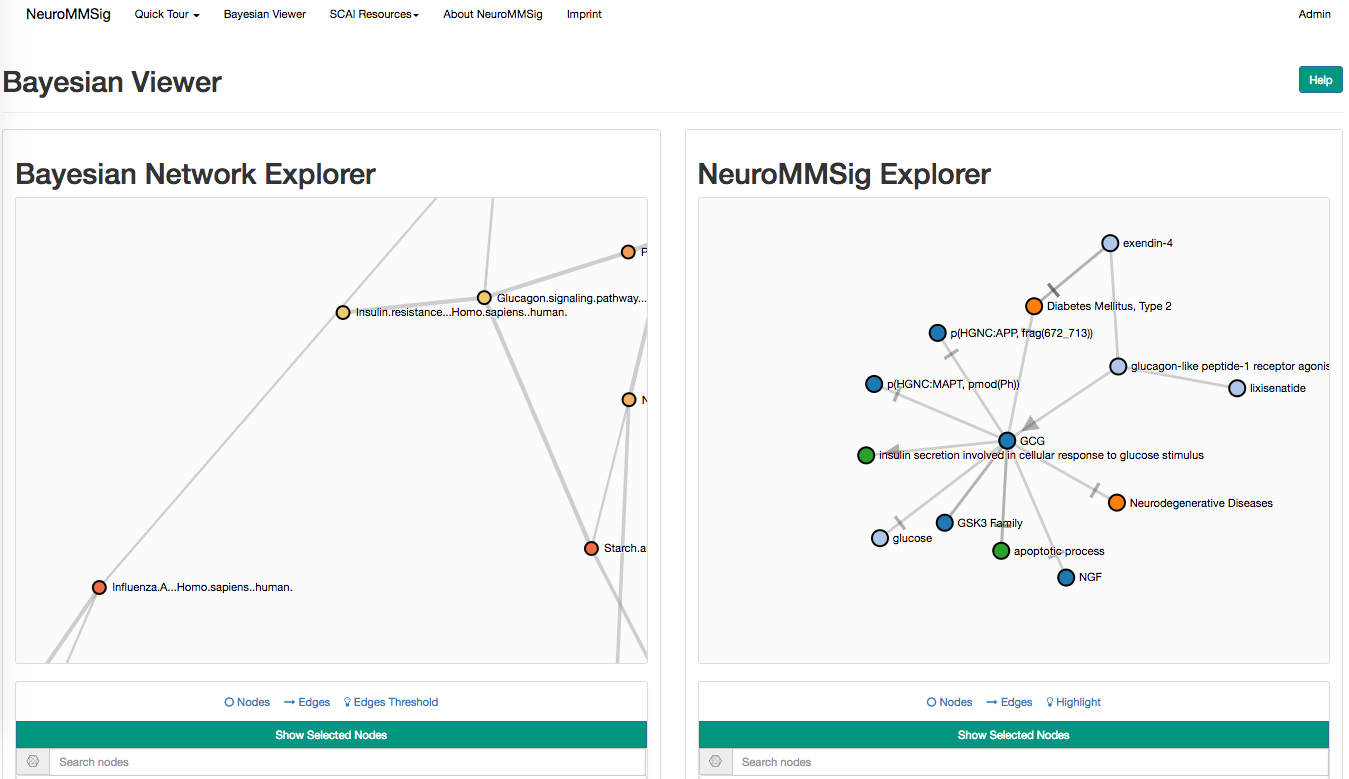
\includegraphics[width=160mm]{images/bayesian_viewer.png}}
\caption[PyBEL Integration with the NeuroMMSig Bayesian Network Explorer]{As an addition to the \ac{NeuroMMSig} Mechanism Enrichment Server, bayesian modeling techniques are used to analyze the dependencies of clinical variables, mapped to \ac{NeuroMMSig} subgraphs, and displayed in a multi-scale exploration environment using the underlying PyBEL visualization system.}
\label{Fig:bayesian_viewer}
\end{figure}

\begin{figure}
\captionsetup{format=plain}
\makebox[\textwidth]{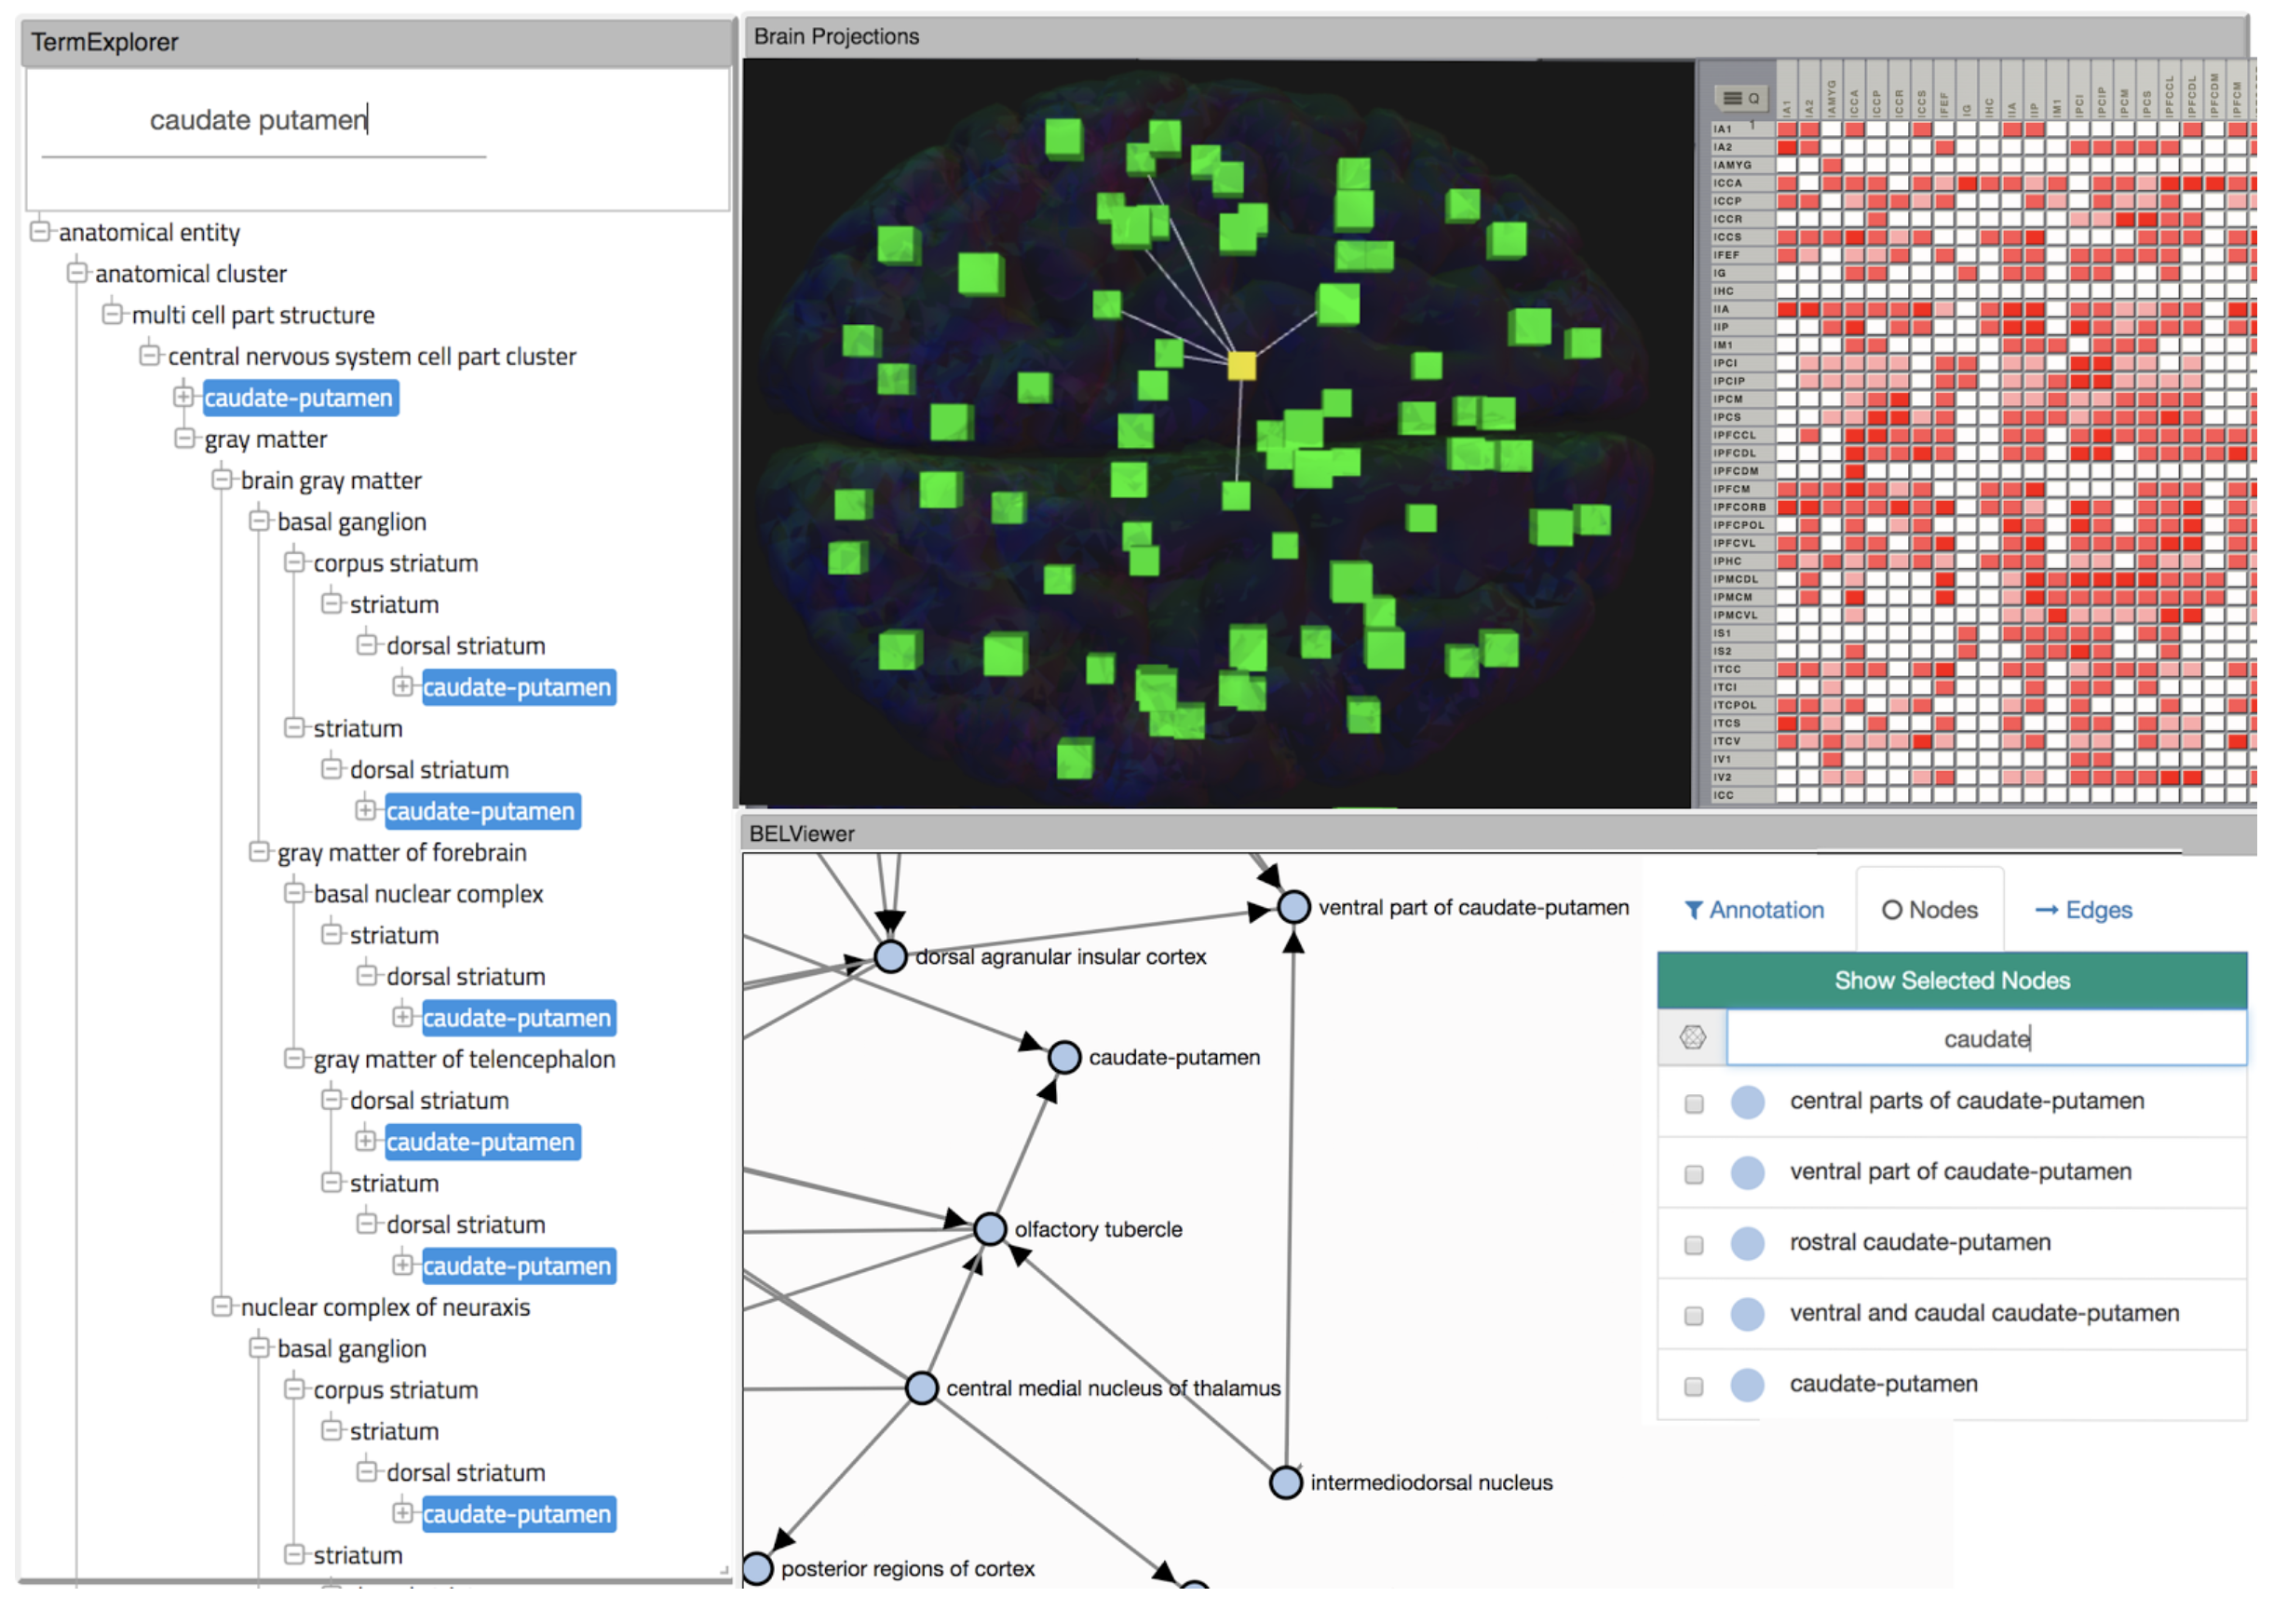
\includegraphics[width=160mm]{images/integration_tvb.png}}
\caption[PyBEL Integration with The Virtual Brain]{The PyBEL visualization system is linked to the tree browser from the Ontology Lookup Service \cite{Cote2006} and connectivity viewer from The Virtual Brain \cite{Leon2013} to allow for interactive exploration of the knowledge related to given brain regions as well as their undirected connectivity or directed projection information.}
\label{Fig:integration_tvb}
\end{figure}

\section{Remarks on Development}

\subsection{Software Stability}

This software was developed under a test-driven development cycle, where extensive unit tests were written to check the stability of the many functions that make up the five components of the software. The procedure for running these tests is encoded with the \verb|tox| build system that is automatically run by Travis \ac{CI} (https://travis-ci.org) upon each push of code to GitHub (https://github.com). The coverage of these tests are then assessed by CodeCov (https://codecov.io).

\subsection{Installation and Usability}

Travis CI also integrates with the "tags and releases" aspect of GitHub to enable automatic build of the code and distribution through PyPI (https://pypi.org), the main packaging system for Python. All relevant information for installation is bundled in the package, so it can be installed with zero configuration on any computer using \verb|pip install pybel| from any terminal, on any operating system, running any modern version of the Python programming language. Finally, the documentation for PyBEL is included in its repository and is automatically built with Sphinx (http://www.sphinx-doc.org) and uploaded to Read the Docs (https://readthedocs.org) upon each push of code to GitHub.

\section{Discussion}

\subsection{Extensibility of Syntax}

Even after its v2.0 update, the \ac{BEL} specification does not yet explicitly specify many concepts in molecular biology such as epigenetic information (e.g. methylation), which is a crucial part of modeling of complex diseases \cite{Irin2015}. The inevitability of language evolution prompted the development of the parser in modules so that new syntax could be proposed and implemented quickly. As a proof of concept, a syntax extension for gene modifications is included in the package by default.

\subsection{Extensibility of Resources}
Historically, \ac{BEL} namespace files have used a custom definition format; but the creation and maintenance of terminologies in the biological domain has tended towards the usage of \ac{OWL}. Furthermore, many namespaces such as dbSNP \cite{Sherry2001} are growing too large to enumerate during semantic integration and validation. The modular architecture of the PyBEL parser enables easy implementation of new definition file formats, external validation services, or even alternative schemes for definition statements to address these issues.

PyBEL introduces syntax for defining namespaces with a consistent pattern using a regular expression to overcome this issue. For these namespaces, semantic validation can be perform in post-processing against the underlying database. The dbSNP namespace can be defined with a syntax familiar to BEL annotation definitions with regular expressions as follows:

\verb|DEFINE NAMESPACE dbSNP AS PATTERN "rs[0-9]+"|

\subsection{Integration of Data}

While \ac{BEL} is often used to formalize knowledge curated from unstructured sources, PyBEL also accommodates the integration of knowledge from structured sources. Existing solutions for resolving equivalences across namespaces have relied on the creation and external hosting of extensive lookup tables. PyBEL could take inspiration from the \ac{OWL} format and enable equivalency information to be directly integrated in a network as edges. 

Again, the parser is extensible enough to implement dedicated syntax for equivalency similar to the standard syntax for gene orthology (\verb|orthologousTo|), protein complex component definitions (\verb|hasComponent|), and protein family membership (\verb|hasMember|). This is realized with the addition of the \verb|equivalentTo| relation, which can be reasoned over using network algorithms directly or collapsed for further use. For example, the fragments produced by amyloid cleavage can be represented in \ac{BEL} with either a protein and fragment combination, or referred directly by its entry in \ac{ChEBI} \cite{Hastings2013}. With the PyBEL extension, this can be written as:

\verb|p(HGNC:APP, frag(672_713)) equivalentTo \|

\verb|a(CHEBI:"amyloid-beta polypeptide 40")|

The hierarchical information encoded in ontologies can also be directly integrated. For example, integrating the \ac{ChEBI} Ontology could allow for reasoning over its multiple functional and structural hierarchies of chemical space. These entries can enable mechanistically-focused chemical repurposing strategies by identifying links between chemical inhibitors in disparate regions of a network \cite{Hastings2013}. 

\subsection{Inaccessible Formats}

Data locked away in other formats such as BioPax and SBML cannot be accessed by PyBEL currently. Development of knowledge assemblers, like \ac{INDRA} \cite{indra}, provide support for import of many formats. PyBEL will enable the import of \ac{BEL} documents much more quickly, and ultimately enable the export of \ac{SBML}. In the future, it would also be useful to develop additional interchange tools for \ac{BioPAX} to \ac{BEL}, but this is a large task that will be limited by the expressibility of each language and the difficult development of a two-way mapping.
There is ongoing work on integrating PyBEL and \ac{INDRA} to immediately make accessible the text mining results from REACH \cite{Valenzuela-Escarcega2015} and TRIPS \cite{Allen2008} as well as the prior knowledge sources assembled for the \ac{INDRA} workflow. Future work is planned to integrate the \ac{BELIEF} workflow \cite{Madan2016} as well.

\subsection{Comparison with Previous Software}

After describing PyBEL, Table 3 is used to make a direct feature comparison with the OpenBEL Framework and bel.rb. While the OpenBEL Framework has some features that are still in develop in the PyBEL ecosystem (see following section on Bio2BEL), PyBEL is the most feature complete and robust option.

\begin{table}
\centering
\caption[BEL Software Ecosystem Comparison]{A comparison of the available software for processing \ac{BEL}. *To the best of our ability, we were unable to install bel.rb using its documentation and unsuccessful in soliciting support through GitHub or OpenBEL's proposed channel of communication on Gitter (https://gitter.im/OpenBEL/chat)}
\label{tab:comparison}
\def\arraystretch{1.1}
\begin{tabular}{p{4cm} p{4cm} p{4cm} p{4cm}}
 & OpenBEL Framework & bel.rb & PyBEL \\
\hline
Programming Language & Java & Ruby & Python \\
Latest Official Release & 2015-06-11 & 1.1.2 - 2017-05-22 & 0.9.0 - 2017-09-19 \\
Installation & Not available on package manager such as brew or apt-get & \verb|gem install bel|* & \verb|pip install pybel| \\
BEL 2.0 Support & No & Experimental & Yes \\
Testing & Yes & Yes & Yes \\
Continuous Integration & No & Yes & Yes \\
Code Quality Testing & No & No & CodeCov and Code Climate \\
Documentation and Tutorials & No & Yes & Yes \\
Command Line Interface & Yes & Yes & Yes \\
Import & BEL Script & BEL Script, RDF & See Table 1 \\
Export & KAM Navigator & RDF & See Tables 1 and 2 \\
Visualization & KAM Navigator & None & See Figures 6-8 \\
Namespace Formats & BELNS & BELNS & BELNS and OWL \\
Compilation Process & Orthology, Named Complexes, Central Dogma & None & Central Dogma \\
Explicit Equivalence Handling & Yes & No & No \\
Extensible Parser & No & No & Yes \\
Programmatic API & No & No & Yes \\
Caching Mechanism & Yes & Yes & Yes \\
Internal DSL & No & Yes & No \\
Ongoing Development & No & No & Yes
\end{tabular}
\end{table}

\section{Conclusions}

\subsection{Applications in Re-curation}
The \ac{NeuroMMSig} knowledge assemblies for \ac{AD} and \ac{PD} had many syntactic, semantic, and biological errors. The PyBEL parser provides a much more useful error analysis than previous software and immediately enabled fixes for many of the syntactic and semantic errors. During this process, a preliminary version control process was implemented to track progress over time. With less than 200 commits and over a period of six months, 5327 of the 8030 errors in the Alzheimer's disease knowledge assembly and 465 of the 1171 errors in the Parkinson's disease knowledge assembly were fixed (Figure 12).

\begin{figure}
\captionsetup{format=plain}
\makebox[\textwidth]{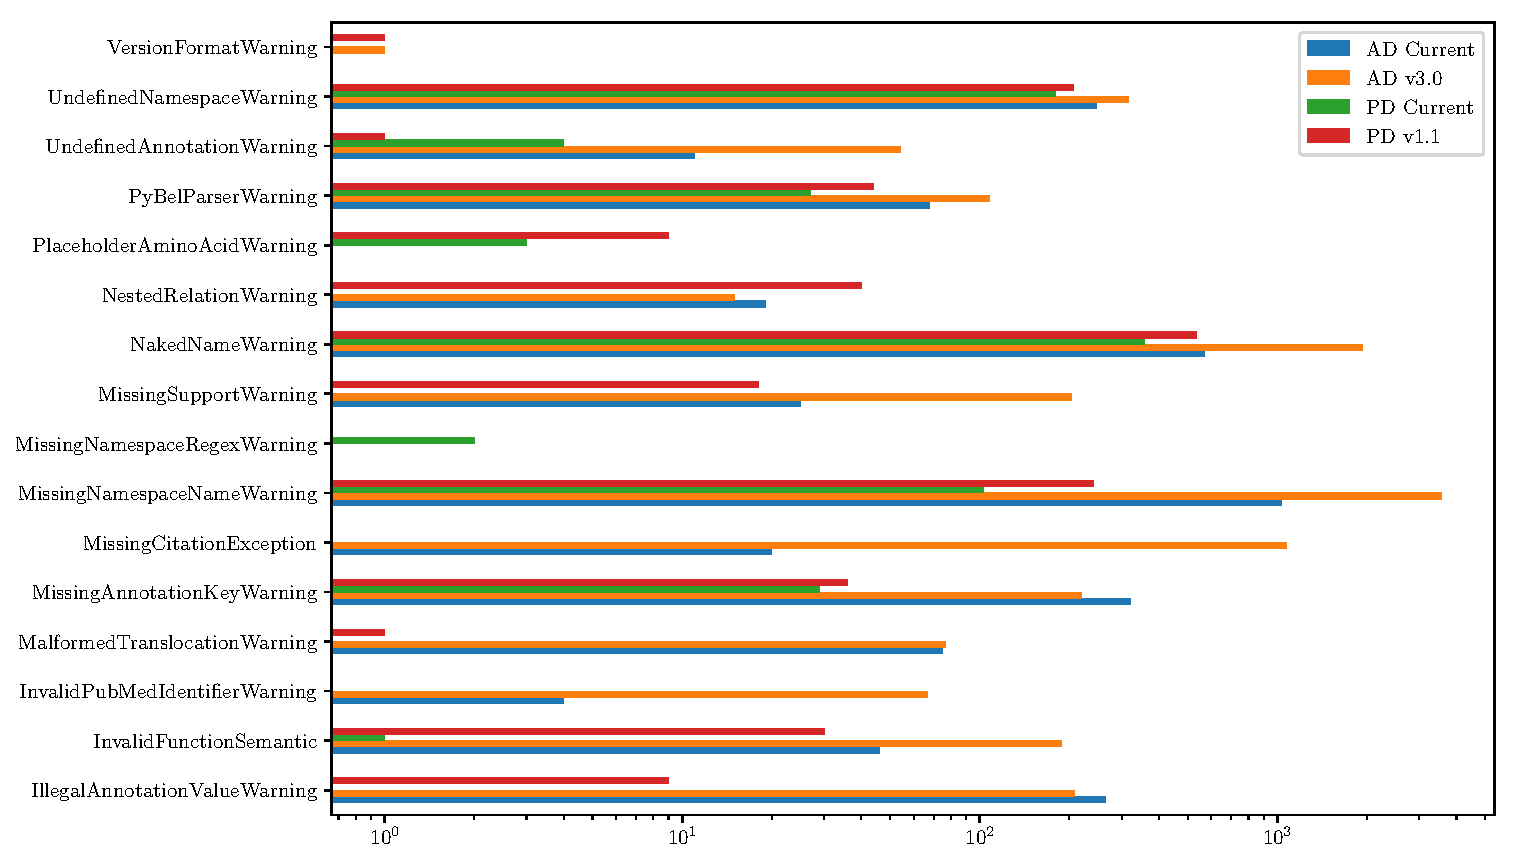
\includegraphics[width=160mm]{images/recuration_bars.pdf}}
\caption[NeuroMMSig Recuration Summary]{The re-curation efforts of the Alzheimer's disease and Parkinson's disease knowledge assemblies showed significant progress after the introduction of PyBEL.}
\label{Fig:recuration_summary}
\end{figure}

Biological problems are much more difficult to detect a priori, but later sections in this thesis describe how integrating data from external sources could allow for an assessment of the "biological grammar" underlying the knowledge assemblies. Future integration with \ac{INDRA} can provide the first steps in automatic analysis of biological correctness using its belief propagation algorithm for quantifying the reliability of statements  based on consensus across text mining and a-priori knowledge bases.

\subsection{Applications in Psychology and Psychiatry}

PyBEL has already been used to stretch the boundaries of manual curation. Projects dealing with anxiety and anhedonia have led to the curation of neuronal connectivity and projects. Other projects dealing with \ac{PTSD} and \ac{TBI} have led to a much larger focus on the curation of biological processes, phenotypes, and clinical measurements. The limited information on the molecular level combine with the focus on non-molecular clinical measurements in these domains motivates the need for integration of new a-priori knowledge bases to assist in the contextualization of new information, critical assessment of the completeness and correctness of new curated material, and new analytical techniques.

\subsection{Future Work}

Integrating chemical information systems like the Comparative Toxicogenomics Database \cite{Davis2017} could enable a previously envisioned chemoinformatics platform \cite{Emon2017} backed by the mechanistic knowledge encoded in \ac{BEL} networks. The extensibility of the network data container enables the integration of relations that are not explicitly defined by \ac{BEL}, such as weighted chemical similarities, for development of novel algorithms and analyses as well as enables the implementation of previously published algorithms for more general use. 
